\documentclass[conference]{IEEEtran}
\IEEEoverridecommandlockouts
\usepackage{cite}
\usepackage{amsmath,amssymb}
\usepackage{graphicx}
\usepackage{booktabs}
\usepackage{url}
\usepackage{balance}

\title{A Reduced-Scale Study of GOPIM: Selective Vertex Updates and Analytical Pipeline Evaluation}

\author{
\IEEEauthorblockN{Deepit Gupta, Lakshay Bansal, Pratyush, and Sanjeev}
}

\begin{document}
\maketitle

\begin{abstract}
Processing-in-memory (PIM) can accelerate graph convolutional network (GCN)
training, but skewed graph degrees and stage durations complicate data
placement and pipeline scheduling. This report implements a reduced-scale
software study inspired by GOPIM. We train graph convolutional networks on
Cora and CiteSeer with degree-based interleaved selective updating (ISU), a
new loss-aware update policy, and a full-update control. We also compare
serial, static equal-replica, and GOPIM-style greedy resource allocation using
an analytical crossbar timing and array-energy model. In one 50-epoch,
single-seed run, both selective policies use about 19.2\% fewer modeled
vertex updates than full updating. Accuracy effects are mixed: loss-aware ISU
is lower than degree ISU on Cora and slightly higher on CiteSeer. The
analytical pipeline model predicts slower pipelined schedules than its serial
baseline and equal array energy by construction. These results are not a
numerical reproduction of the paper; we explain the workload, simulator, and
resource-model differences that prevent direct comparison.
\end{abstract}

\begin{IEEEkeywords}
graph neural networks, processing-in-memory, selective updating, analytical
model, pipeline scheduling
\end{IEEEkeywords}

\section{Introduction}
Graph convolutional networks (GCNs) combine feature transformation and
neighborhood aggregation. Irregular graph structure makes aggregation and
data movement expensive, motivating processing-in-memory (PIM) accelerators.
The original GCN formulation established the propagation model used in this
study~\cite{kipf2017gcn}. Prior PIM work such as ISAAC explored in-situ analog
arithmetic in resistive crossbars~\cite{shafiee2016isaac}, while graph-specific
accelerators such as HyGCN use a hybrid architecture for GCN workloads~\cite{yan2020hygcn}.
GOPIM addresses crossbar underutilization with stage-aware replica allocation
and interleaved selective vertex updating (ISU)~\cite{yang2025gopim}.

This project follows the reduced-scale assignment: implement GCN training on
two small graphs, apply adaptive selective updating, report accuracy, and
compare serial, SlimGNN-like, and GOPIM-style pipeline allocations. It also
evaluates one additional policy: ranking labeled vertices partly by their
previous-epoch training loss while preserving ISU's update budget.

The scope is deliberately a software and analytical model. It does not
execute the upstream NeuroSim simulator, large OGB workloads, or real
hardware. Accordingly, the main contribution of this report is a transparent
implementation and a reproducible comparison, not a claim of hardware
performance parity with GOPIM.

\section{Background and Study Questions}
\subsection{GOPIM Techniques}
GOPIM divides an $L$-layer GCN training iteration into $4L$ stages:
combination (CO), aggregation (AG), layer-error calculation (LC), and
gradient calculation (GC). Its pipeline overlaps micro-batches and allocates
crossbar replicas to reduce stage imbalance. Its ISU policy sorts vertices by
degree, updates important vertices every epoch, and updates less-important
vertices every 20 epochs. The paper selects an adaptive update fraction based
on graph density and evaluates a 64-vertex micro-batch by default~\cite{yang2025gopim}.

\subsection{Questions}
We study three questions:
\begin{enumerate}
  \item Can the reduced-scale training path preserve test accuracy while
  lowering the modeled count of vertex updates?
  \item Does loss-aware ranking improve accuracy over degree-only ISU under
  the same update budget?
  \item Do the simplified pipeline estimates reproduce the qualitative
  speedup and energy trends reported by GOPIM?
\end{enumerate}

\section{Implementation}
\subsection{Graph Model and Training}
The implementation uses PyTorch and PyTorch Geometric~\cite{fey2019pyg}.
For node $v$, a graph-convolution layer computes the normalized propagation
\begin{equation}
  H^{(\ell+1)} =
  \sigma\!\left(\widetilde{D}^{-1/2}\widetilde{A}
  \widetilde{D}^{-1/2} H^{(\ell)} W^{(\ell)}\right),
\end{equation}
where $\widetilde{A}=A+I$, $\widetilde{D}$ is its degree matrix, $W^{(\ell)}$
is a learned weight matrix, and $\sigma$ is ReLU. We use the Planetoid Cora
and CiteSeer node-classification graphs and their standard train, validation,
and test masks~\cite{yang2016planetoid}. The model uses two layers, 64 hidden
channels, dropout 0.5, Adam with learning rate 0.01, and 50 epochs. The
experiment uses seed 42 and CPU execution.

\subsection{Degree-Based ISU}
Let $\bar d$ be the graph's average degree. The policy selects the highest
degree 80\% of vertices when $\bar d\leq 8$ and 50\% otherwise. Selected
vertices update every epoch; unselected vertices update every 20 epochs.
Gradients for non-updating vertices are masked in the GCN representation.
Because both tested graphs are sparse, both use the 80\% threshold.

\subsection{New Policy: Loss-Aware ISU}
To test whether update work should follow current training difficulty as well
as structural importance, we add loss-aware ISU. At the end of each epoch,
per-vertex training loss is computed for labeled training vertices. At the
next epoch, observed vertices are ranked by loss and degree; their combined
score is
\begin{equation}
  s_v = 0.75\,r_{\mathrm{loss}}(v)
      + 0.25\,r_{\mathrm{degree}}(v),
\end{equation}
where each $r$ is a normalized descending rank. Vertices without a training
label use degree rank only. The policy selects the same number of vertices
as degree ISU and retains the every-20-epoch update of all vertices. Thus,
the new policy changes selection, not the configured update budget. This is
an experimental extension, not a technique claimed by the GOPIM paper.

\subsection{Analytical Pipeline Model}
The pipeline comparator evaluates serial reuse of the full modeled
crossbar budget, an equal-replica static pipeline proxy, and the GOPIM greedy
bottleneck allocator. The modeled architecture has 64$\times$64, 2-bit
crossbars, a 128-KiB global buffer, 29.31-ns read pulses, and 50.88-ns write
pulses. Its 65,536 virtual tiles, eight PEs per tile, and 32 crossbars per PE
correspond to 16,777,216 crossbars (16 GiB at the modeled cell density).
These are resource counts, not instantiated objects.

The reported latency is a crossbar-pulse floor, not full accelerator
latency. The first-order read-energy estimate adapts a line-capacitance
switching model; the write estimate combines cell and line energy. It assumes
50\% active read rows, one pulse for every cell in a fully updated 64-cell
row, and the mean of the on/off cell resistances. Both estimates exclude
peripheral circuits, buffer and interconnect activity, leakage, idle power,
and replica-copy cost. Total array energy is held constant across allocation
schemes; this model therefore cannot predict allocation-dependent energy
savings.

\section{Experimental Method}
The training comparison runs the same data splits, seed, model dimensions,
optimizer, and epoch count for three conditions: degree ISU, loss-aware ISU,
and full updates. Test accuracy is reported from the final epoch; no
hyperparameter search is performed. The update-count comparison counts
modeled vertices updated across epochs and is not a measured count of physical
ReRAM writes.

Pipeline timings are computed separately from the training wall-clock time.
The comparator schedules four micro-batches using the configured stage
latencies and allocated replica counts. We report makespan relative to the
model's serial baseline. The static equal-replica strategy is explicitly a
proxy rather than an implementation of the original SlimGNN.

\section{Results}
\subsection{Training Accuracy and Update Work}
Table~\ref{tab:training} reports final test accuracy and update counts.
Degree ISU exceeds the full-update score on Cora by 1.4 percentage points;
loss-aware ISU is 0.4 points below full updating on that run. On CiteSeer,
loss-aware ISU is 0.1 points above full updating and 0.2 points above degree
ISU. Each selective policy uses about 19.2\% fewer modeled vertex updates
than full updating. The one-seed differences do not establish statistical
significance.

\begin{table}[t]
\caption{Final Test Accuracy and Modeled Vertex Updates}
\label{tab:training}
\centering
\footnotesize
\begin{tabular}{llrr}
\toprule
Dataset & Policy & Accuracy & Updates \\
\midrule
Cora & Full update & 79.0\% & 135,400 \\
Cora & Degree ISU & 80.4\% & 109,432 \\
Cora & Loss-aware ISU & 78.6\% & 109,432 \\
\midrule
CiteSeer & Full update & 64.3\% & 166,350 \\
CiteSeer & Degree ISU & 64.2\% & 134,430 \\
CiteSeer & Loss-aware ISU & 64.4\% & 134,430 \\
\bottomrule
\end{tabular}
\end{table}

Fig.~\ref{fig:training} visualizes the accuracy and update-count tradeoff.
The new policy does not consistently improve upon degree ISU: it decreases
Cora accuracy by 1.8 points relative to degree ISU, while increasing
CiteSeer accuracy by 0.2 points. The policy meets its fixed update budget on
both datasets.

\begin{figure*}[t]
\centering
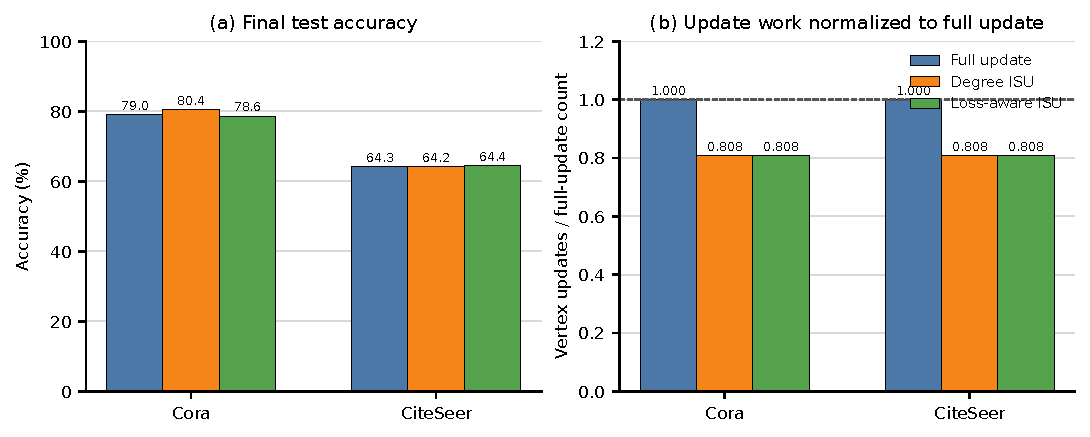
\includegraphics[width=0.94\textwidth]{figures/training_results.pdf}
\caption{Final test accuracy and cumulative modeled vertex updates. Selective
policies use approximately 80.8\% of the full-update count on each graph.}
\label{fig:training}
\end{figure*}

\subsection{Pipeline Comparison}
Table~\ref{tab:pipeline} reports model makespans. In this analytical setup,
the static proxy and GOPIM allocator both take longer than the serial model:
GOPIM is 1.61$\times$ serial time for Cora and 2.24$\times$ for CiteSeer.
The model assigns all three schemes identical energy per dataset (1.515 mJ
for Cora, 4.784 mJ for CiteSeer), so it does not reproduce the paper's energy
reduction trend.

\begin{table}[t]
\caption{Analytical Pipeline Model Results}
\label{tab:pipeline}
\centering
\footnotesize
\begin{tabular}{llrr}
\toprule
Dataset & Allocation & Makespan ($\mu$s) & $T/T_{\mathrm{serial}}$ \\
\midrule
Cora & Serial & 3.787 & 1.000 \\
Cora & Static equal-replica & 5.563 & 1.469 \\
Cora & GOPIM greedy & 6.087 & 1.607 \\
\midrule
CiteSeer & Serial & 19.286 & 1.000 \\
CiteSeer & Static equal-replica & 38.012 & 1.971 \\
CiteSeer & GOPIM greedy & 43.116 & 2.236 \\
\bottomrule
\end{tabular}
\end{table}

\begin{figure*}[t]
\centering
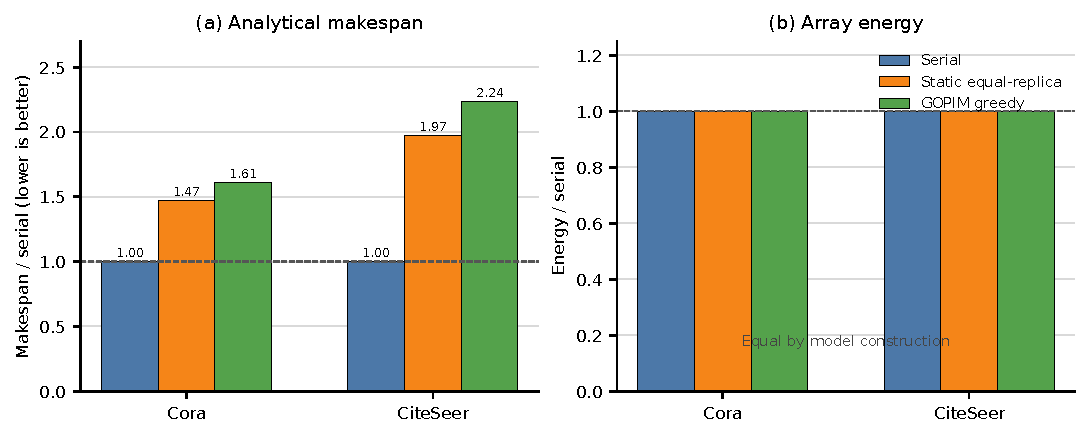
\includegraphics[width=0.94\textwidth]{figures/pipeline_results.pdf}
\caption{Analytical pipeline makespan and array energy normalized to the
serial model. Lower makespan is better; energy is equal across allocation
schemes by construction.}
\label{fig:pipeline}
\end{figure*}

\section{Comparison with the GOPIM Paper}
The paper reports GOPIM outperforming its evaluated baselines, with
10.2$\times$--3454.3$\times$ speedups over Serial across five OGB workloads
and an average 4.0$\times$ energy reduction in its overall comparison
(Fig.~13)~\cite{yang2025gopim}. Its technique ablation reports progressively
improved execution time after pipelining, ISU, and learned allocation
(Fig.~14). The accuracy effect of ISU varies by graph (Table~V). These
directions are not reproduced by our analytical pipeline model, which
predicts slowdown and equal energy.

The difference is expected from the model and workload scope, not evidence
against the paper. First, the paper evaluates OGB workloads~\cite{hu2020ogb} and Cora, whereas
our training experiment uses Cora and CiteSeer; CiteSeer is not a paper
benchmark. Second, the paper's Cora configuration uses three layers and 256
hidden channels, while our run uses two layers and 64 hidden channels.
Third, paper timings come from a detailed PIM simulator, while our pipeline
uses pulse-time floors and omits peripheral, buffering, interconnect, and idle
effects. Fourth, our serial comparator reuses the full crossbar budget for
each stage, whereas the paper's DDI serial mapping uses one replica per
stage. Finally, the SlimGNN-like row is only a static equal-replica proxy.
The numerical speedups, energy values, and baselines are therefore not
directly comparable.

The paper reports that Cora ISU incurs a 0.28\% accuracy loss in its sparse
graph study. Our degree ISU is 1.4 percentage points above the local
full-update control, and loss-aware ISU is 0.4 points below it. Different
model dimensions, training recipes, initialization, and evaluation conditions
prevent interpreting this discrepancy as a reproduction or contradiction.
One seed also makes these local accuracy differences noisy.

\section{Limitations and Reproducibility}
This implementation intentionally omits the upstream NeuroSim source and
runtime integration, full circuit/peripheral models, large graph experiments,
and real hardware. Pipeline energy is a first-order array estimate, not a
measured system energy. The serial resource definition and static pipeline
proxy differ from the paper's baselines. Only one seed and 50 epochs were
used; there are no confidence intervals or multiple-run significance tests.
Thus, the study supports only local observations about accuracy and modeled
update counts, not a claim that the new policy is superior or that paper-level
speedup/energy results have been reproduced.

The ZIP accompanying this report includes the LaTeX source, bibliography,
result CSVs, plotting script, and generated vector figures. To reproduce the
plots, run \texttt{python make\_figures.py} from the source directory. Compile
on Overleaf with the IEEE conference template, or locally with
\texttt{pdflatex}, \texttt{bibtex}, and two additional \texttt{pdflatex} runs.

\section{Conclusion}
We implemented the reduced-scale GCN/ISU and analytical pipeline comparison
and added a loss-aware policy that preserves ISU's modeled update budget. In
one seed, both selective policies reduce modeled update counts by about
19.2\%, while the new policy's accuracy impact is mixed. The analytical
pipeline model fails to reproduce GOPIM's reported speedup and energy trends;
its simplified timing, energy, and baseline assumptions explain why the
comparison is not numerically equivalent. Multi-seed training and a
validated cycle- and energy-level simulator integration would be needed for
stronger conclusions.

\balance
\bibliographystyle{IEEEtran}
\bibliography{references}
\end{document}
